\documentclass[notes,11pt, aspectratio=169, xcolor=table]{beamer}

\usepackage{pgfpages}
% These slides also contain speaker notes. You can print just the slides,
% just the notes, or both, depending on the setting below. Comment out the want
% you want.
\setbeameroption{hide notes} % Only slide
%\setbeameroption{show only notes} % Only notes
%\setbeameroption{show notes on second screen=right} % Both

\usepackage{helvet}
\usepackage[default]{lato}
\usepackage{array}
\usepackage[utf8]{inputenc} 

\newtheorem{proposition}{Proposition}

\usepackage{tikz}
\usetikzlibrary{shapes.geometric}
\usepackage{pgfplots}
\usepackage{graphicx}
\usepackage{verbatim}
\setbeamertemplate{note page}{\pagecolor{yellow!5}\insertnote}
\usetikzlibrary{positioning}
\usetikzlibrary{snakes}
\usetikzlibrary{calc}
\usetikzlibrary{arrows}
\usetikzlibrary{decorations.markings}
\usetikzlibrary{shapes.misc}
\usetikzlibrary{matrix,shapes,arrows,fit,tikzmark}
\usepackage{amsmath}
\usepackage{mathpazo}
\usepackage{hyperref}
\usepackage{lipsum}
\usepackage{multimedia}
\usepackage{graphicx}
\usepackage{multirow}
\usepackage{graphicx}
\usepackage{dcolumn}
\usepackage{bbm}
\usepackage[style=authoryear,sorting=nyt,uniquename=false]{biblatex}
\newcommand{\blue}[1]{\textcolor{blue}{#1}}
\newcommand{\white}[1]{\textcolor{white}{#1}}

\addbibresource{references.bib} 

\newcolumntype{d}[0]{D{.}{.}{5}}

\def\@@mybluebox[#1][#2]#3{
    \sbox\mytempbox{#3}%
    \mytemplen\ht\mytempbox
    \advance\mytemplen #1\relax
    \ht\mytempbox\mytemplen
    \mytemplen\dp\mytempbox
    \advance\mytemplen #2\relax
    \dp\mytempbox\mytemplen
    \colorbox{myblue}{\hspace{1em}\usebox{\mytempbox}\hspace{1em}}}


\usepackage{changepage}
\usepackage{appendixnumberbeamer}
\newcommand{\beginbackup}{
   \newcounter{framenumbervorappendix}
   \setcounter{framenumbervorappendix}{\value{framenumber}}
   \setbeamertemplate{footline}
   {
     \leavevmode%
     \hline
     box{%
       \begin{beamercolorbox}[wd=\paperwidth,ht=2.25ex,dp=1ex,right]{footlinecolor}%
%         \insertframenumber  \hspace*{2ex} 
       \end{beamercolorbox}}%
     \vskip0pt%
   }
 }
\newcommand{\backupend}{
   \addtocounter{framenumbervorappendix}{-\value{framenumber}}
   \addtocounter{framenumber}{\value{framenumbervorappendix}} 
}


\usepackage{graphicx}
\usepackage[space]{grffile}
\usepackage{booktabs}

% These are my colors -- there are many like them, but these ones are mine.
\definecolor{blue}{RGB}{0,114,178}
\definecolor{red}{RGB}{213,94,0}
\definecolor{yellow}{RGB}{240,228,66}
\definecolor{green}{RGB}{0,158,115}

\hypersetup{
  colorlinks=false,
  linkbordercolor = {white},
  linkcolor = {blue}
}


%% I use a beige off white for my background
\definecolor{MyBackground}{RGB}{255,253,218}

%% Uncomment this if you want to change the background color to something else
%\setbeamercolor{background canvas}{bg=MyBackground}

%% Change the bg color to adjust your transition slide background color!
\newenvironment{transitionframe}{
  \setbeamercolor{background canvas}{bg=yellow}
  \begin{frame}}{
    \end{frame}
}

\setbeamercolor{frametitle}{fg=blue}
\setbeamercolor{title}{fg=blue}
\setbeamertemplate{footline}[frame number]
\setbeamertemplate{navigation symbols}{} 
\setbeamertemplate{itemize items}{-}
\setbeamercolor{itemize item}{fg=blue}
\setbeamercolor{itemize subitem}{fg=blue}
\setbeamercolor{enumerate item}{fg=blue}
\setbeamercolor{enumerate subitem}{fg=blue}
\setbeamercolor{button}{bg=MyBackground,fg=blue,}



% If you like road maps, rather than having clutter at the top, have a roadmap show up at the end of each section 
% (and after your introduction)
% Uncomment this is if you want the roadmap!
% \AtBeginSection[]
% {
%    \begin{frame}
%        \frametitle{Roadmap of Talk}
%        \tableofcontents[currentsection]
%    \end{frame}
% }
\setbeamercolor{section in toc}{fg=blue}
\setbeamercolor{subsection in toc}{fg=red}
\setbeamersize{text margin left=1em,text margin right=1em} 

\newenvironment{wideitemize}{\itemize\addtolength{\itemsep}{10pt}}{\enditemize}

\usepackage{environ}
\NewEnviron{videoframe}[1]{
  \begin{frame}
    \vspace{-8pt}
    \begin{columns}[onlytextwidth, T] % align columns
      \begin{column}{.58\textwidth}
        \begin{minipage}[t][\textheight][t]
          {\dimexpr\textwidth}
          \vspace{8pt}
          \hspace{4pt} {\Large \sc \textcolor{blue}{#1}}
          \vspace{8pt}
          
          \BODY
        \end{minipage}
      \end{column}%
      \hfill%
      \begin{column}{.42\textwidth}
        \colorbox{green!20}{\begin{minipage}[t][1.2\textheight][t]
            {\dimexpr\textwidth}
            Face goes here
          \end{minipage}}
      \end{column}%
    \end{columns}
  \end{frame}
}

\title[]{International Trade: Lecture XX}
\subtitle[]{Firms and Trade: The Krugman Model}
\author[Góes]
{Carlos Góes\inst{1}}
\date{Fall 2025}
\institute[GWU]{\inst{1} George Washington University }



\begin{document}

%%% TIKZ STUFF
\tikzset{   
        every picture/.style={remember picture,baseline},
        every node/.style={anchor=base,align=center,outer sep=1.5pt},
        every path/.style={thick},
        }
\newcommand\marktopleft[1]{%
    \tikz[overlay,remember picture] 
        \node (marker-#1-a) at (-.3em,.3em) {};%
}
\newcommand\markbottomright[2]{%
    \tikz[overlay,remember picture] 
        \node (marker-#1-b) at (0em,0em) {};%
}
\tikzstyle{every picture}+=[remember picture] 
\tikzstyle{mybox} =[draw=black, very thick, rectangle, inner sep=10pt, inner ysep=20pt]
\tikzstyle{fancytitle} =[draw=black,fill=red, text=white]
%%%% END TIKZ STUFF



%----------------------------------------------------------------------%
%-------------------       TITLE PAGE       ---------------------------%
%----------------------------------------------------------------------%





%----------------------------------------------------------------------%






%----------------------------------------------------------------------%
%----------------------------------------------------------------------%

%----------------------------------------------------------------------%
\frame{\titlepage}
\addtocounter{framenumber}{-1}
%----------------------------------------------------------------------%

\section{Intro and recap}

\begin{frame}{Takeaways from last class}
\begin{wideitemize}
    \item Demand for differentiated goods
    \item Elasticity of substitution ($\sigma$)
    \item For all good, optimal choice implies MRS = relative prices
    \item Production under monopolistic competition, fixed costs, and IRS = profit opportunities
    \item Monopoly power implies $p^* > MC$
    \item In our framework, prices = mark up over MC.
    \end{wideitemize}
 \end{frame}

 \begin{frame}{Demand functions}
\begin{columns}
    \begin{column}{0.5\textwidth}
       After some algebra, we can solve for demand functions:            
        \begin{equation*}
            q_i(\varphi) = \underbrace{\left( \frac{p_i(\varphi)}{P_i} \right)^{-\sigma}}_{\text{relative price}} \times \underbrace{\frac{I_i}{P_i}}_{\text{real income}}
            \end{equation*}
        {\scriptsize \qquad \textcolor{gray}{(check handout for step by step derivation)}}

       \begin{wideitemize}
        \item<2-> \blue{Intuition}: demand is...
        \begin{itemize}
            \item ...decreasing in the relative price
            \item ...increasing in real aggregate income
        \end{itemize}        

        \item<3-> What about $\sigma$?
        \begin{itemize}
            \item<4-> $\sigma$ small: large change in price, small drop in demand
            \item<5-> $\sigma$ large: small change in price, large drop in demand
        \end{itemize}
        \end{wideitemize}


    \end{column}
    
    \begin{column}{0.5\textwidth}
    \onslide<6->{
    \begin{figure}[htp]
        \centering
        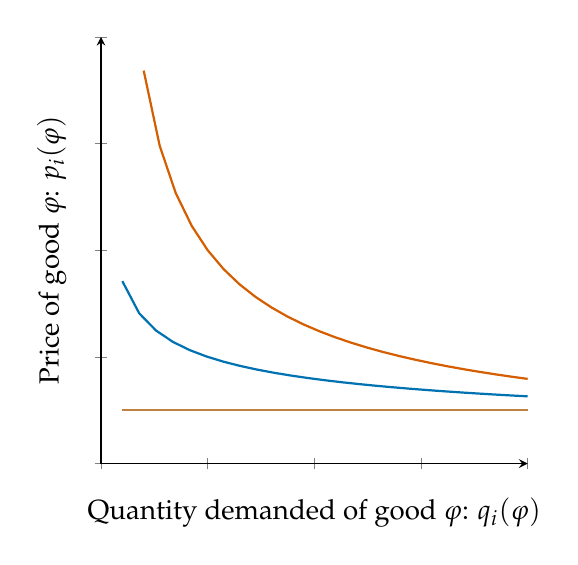
\begin{tikzpicture}
        \pgfmathsetmacro{\sigmaa}{1.5}
        \pgfmathsetmacro{\sigmab}{3}
        \pgfmathsetmacro{\sigmac}{10000000}
        \pgfmathsetmacro{\P}{0.25}
        \pgfmathsetmacro{\I}{1}
        
        \centering
        \begin{axis}[
            ylabel={Price of good $\varphi$: $p_i(\varphi)$},
            xlabel={Quantity demanded of good $\varphi$: $q_i(\varphi)$},
            ymin=0, ymax=2,
            xmin=0, xmax=2,
            yticklabel=\empty,
            xticklabel=\empty,
            axis lines=left,
            enlargelimits=false,
            clip=false,
            axis on top,
            scaled x ticks=false,
            width=7cm, height=7cm,
            title style={font=\bfseries}
        ]
        
        % PPF: Q_C = (L/a_C) - (a_R/a_C) * Q_R
    
        
          \addplot[thick,red,  domain=0.2:2]
            {\P * ((x*\P)/\I)^(-1/\sigmaa)};
          \addplot[thick,blue, domain=0.1:2]
            {\P * ((x*\P)/\I)^(-1/\sigmab)};
          \addplot[thick,brown,domain=0.1:2]
            {\P};  % σ → ∞  ⇒  horizontal line at p = P
            
        \end{axis}
    
    \end{tikzpicture}
            \caption{Demand curve with different elasticities: \textcolor{red}{$\sigma=1.5$, \textcolor{blue}{$\sigma=3$}, \textcolor{brown}{$\sigma=\infty$}}}
        \label{fig: ces-demand}
    \end{figure}
    
        }

            \end{column}
\end{columns}
\end{frame}

\begin{frame}{Production}

\begin{wideitemize}
    \item Producers of each good $\varphi$ have a monopoly over the production of their good
    \item They also will have to pay a fixed cost $\bar{f}$ to set up shop (only if they enter the market)

    \item To produce a given quantity $q_i(\varphi)$, labor used is:

    \begin{equation*}
         \ell = \bar{f} + a^*q_i(\varphi) \iff q_i(\varphi) = \frac{1}{a^*} (\ell - \bar{f})
    \end{equation*}

    \item \blue{Optimal price = mark-up $\times$ marginal cost.}
    \begin{eqnarray*}
        p^* &=& \frac{\sigma}{\sigma -1}\times MC 
    \end{eqnarray*}

    \item Note $\frac{\sigma}{\sigma -1} > 1$. We call this a mark-up. \\
    \qquad \textcolor{gray}{(what happens when $\sigma \to \infty$?)}
    \end{wideitemize}
    
\end{frame}

\begin{frame}{Monopolistic competition}
\addtocounter{framenumber}{-1}
\centering
    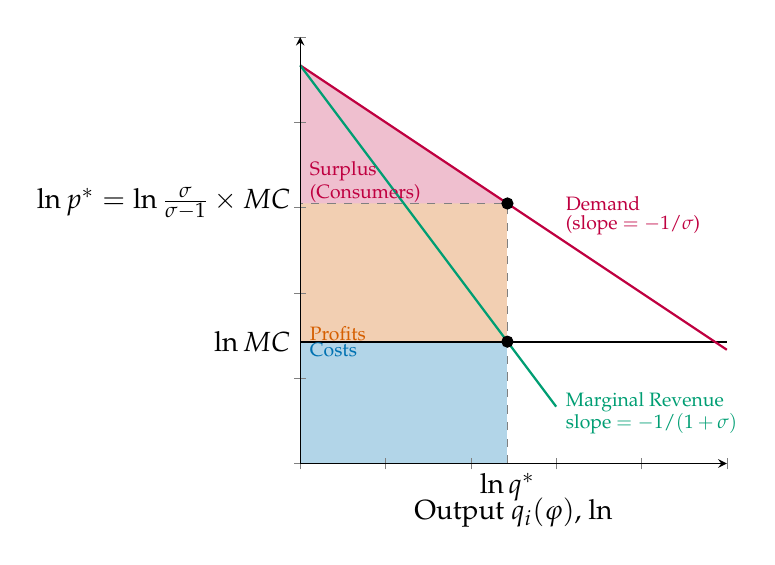
\begin{tikzpicture}
    \pgfmathsetmacro{\K}{7}
    \pgfmathsetmacro{\sigmaa}{1.5}

    \pgfmathsetmacro{\A}{7}
    \pgfmathsetmacro{\b}{0.75}
    \pgfmathsetmacro{\m}{0.35}
    \pgfmathsetmacro{\pmax}{\A/\b}          % choke price  (demand intercept)
    \pgfmathsetmacro{\qc}{\A - \b/\m}       % competitive quantity (P = MC)
        
    
    
    \begin{axis}[
        xlabel={Output $q_i(\varphi)$, ln},
        ymin=0, ymax=10,
        xmin=0, xmax=5,
        yticklabel=\empty,
        xticklabel=\empty,
        axis lines=left,
        enlargelimits=false,
        clip=false,
        axis on top,
        scaled x ticks=false,
        width=7cm, height=7cm,
        title style={font=\bfseries}
    ]

        \pgfmathsetmacro{\q}{((\A / \b - 1/ \m ) / ( 2/\b))}
        \pgfmathsetmacro{\p}{ (\A / \b) - 1/\b * \q }
        % profits
        \addplot[fill=red!30, draw=none] coordinates
            {(0,1/\m) (0,\p) (\q,\p) (\q,1/\m)} -- cycle;
        % costs
        \addplot[fill=blue!30, draw=none] coordinates
            {(0,0) (0,1/\m) (\q,1/\m) (\q,0)} -- cycle;
        % consumer-surplus
        \addplot[fill=purple!25, draw=none] coordinates
            {(0,\p) (0,\pmax) (\q,\p)} -- cycle;
        
            
        \addplot[black, thick, domain=0:5] {1/\m};
        \addplot[purple, thick, domain=0:5] {(\A / \b) - 1/\b * x};
        \addplot[green, thick, domain=0:3] {(\A / \b) - 2/\b * x};
        %\pgfmathsetmacro{\f}{\p * \q - \q / \m}
        %\addplot[blue, thick, domain=1:5] {1/\m + \f / x};

        
        \addplot[gray, dashed] coordinates {(\q,0) (\q,\p) (0,\p)};
        \addplot[only marks, mark=*, color=black, mark size=2pt] coordinates {(\q,\p)};
        \addplot[only marks, mark=*, color=black, mark size=2pt] coordinates {(\q,1/\m)};

        %\addplot[gray, dashed] coordinates {(\q,1/\m + \f / \q) (0,1/\m + \f / \q)};
        %\addplot[only marks, mark=*, color=black, mark size=2pt] coordinates {(\q,1/\m + \f / \q)};

        \node[anchor = south west] at (axis cs: 0,{\p+.3}) {\scriptsize \textcolor{purple}{Surplus}};
        \node[anchor = south west] at (axis cs: 0,{\p-.2}) {\scriptsize \textcolor{purple}{(Consumers)}};
        \node[anchor = south west] at (axis cs: 0,{1/(\m)-.2}) {\scriptsize \textcolor{red}{Profits}};
        \node[anchor = north west] at (axis cs: 0,{1/(\m)+.2}) {\scriptsize \textcolor{blue}{Costs}};

        %\node[anchor=south west] at (axis cs: 5,{1/\m+.43}) {\textcolor{blue}{Average Cost}};
        \node[anchor=west] at (axis cs: 3,\p) {\scriptsize \textcolor{purple}{Demand}};
        \node[anchor=west] at (axis cs: 3,\p-.5) {\scriptsize \textcolor{purple}{(slope $= - 1/\sigma$)}};
        \node[anchor=west] at (axis cs: 3,{1/(2*\m)}) {\textcolor{green}{\scriptsize Marginal Revenue}};
        \node[anchor=west] at (axis cs: 3,{1/(2*\m)-.5}) {\textcolor{green}{\scriptsize slope $= - 1/(1+\sigma)$}};

        \node[anchor=east] at (axis cs: 0,\p) {$\ln p^{*}=\ln \frac{\sigma}{\sigma-1}\times MC$};
        \node[anchor=east] at (axis cs: 0,1/ \m) {$\ln  MC$};

        \node[anchor=north] at (axis cs: \q,0) {$\ln q^*$};

    \end{axis}

    \end{tikzpicture}

 \end{frame}


\begin{frame}{This class}
\begin{wideitemize}
    \item How to solve for the equilibrium of this model?
    \item What are the prices $\{p^*, P_i\}$, quantities demanded $\{q^*,Q_i\}$, goods in eqm $\{N\}$?
    \item What happens once we open up to trade?
    \end{wideitemize}
 \end{frame}

\section{Free entry}

\begin{frame}{Entry into the market}

\begin{wideitemize}
    \item Firms will only enter the market if they expect their profit $\pi_i(\varphi) \ge0$
    \item<2-> If not, they would make a loss, so it would be rational to exit the market.
    \item<3-> But what if profits are (strictly) positive ($\pi_i(\varphi) >0$)?

    \item<4-> Then new entrants could:

    \begin{itemize}
        \item<5-> pay the fixed cost $w_i \bar{f}$
        \item<6-> set up a new shop for a new product
        \item<7-> charge the markup over marginal cost, and
        \item<8-> make a profit!
    \end{itemize}
\end{wideitemize}    
\end{frame}

\begin{frame}{Entry into the market}

    \begin{wideitemize}
    \item New firms will enter the market up to the point in which there is no additional expected profit to be made and $\pi_i(\varphi) =0$.

    \item<2-> What is this point?
    
\begin{eqnarray*}
    \pi_i(\varphi) &=& (p^* - MC) q^* - w_i \bar{f} = 0\\
    &=& \left(\frac{\sigma}{\sigma -1}a^*w_i - a^* w_i\right) q^* - w_i \bar{f} =0  
\end{eqnarray*}

    \item<3-> Solving for $q^*$:

    \begin{equation*}
    \boxed{
        q^* = (\sigma-1) \times \frac{\bar{f}}{a^*}
    }
    \end{equation*}

    (note: quantity sold by firm is identical) 

    \end{wideitemize}
    
\end{frame}

\begin{frame}{Entry into the market}

 
    \begin{equation*}
    \boxed{
        q^* = (\sigma-1) \times \frac{\bar{f}}{a^*}
    }
    \end{equation*}

    \blue{Intuition}:
    \begin{wideitemize}

    \item<2-> $\bar{f}$ controls increasing returns to scale \\
        \qquad (if $\bar{f}$ is high, quantity sold per firm will be higher)

    \item<3-> $\sigma$ controls mark-up (hence, prices) \\
        \qquad (if $\sigma$ is high, prices are low and quantity sold per firm will be higher)

    \item<4-> $a^*$ input labor requirement, maps from labor input to quantities

    \end{wideitemize}
    
\end{frame}

\begin{frame}{Free entry in equilibrium}
    \begin{wideitemize}
        \item A surprising result is that, since all firms are identical, none of them will make positive profits in equilibrium!
        \item They maximize marginal profits, but free-entry + fixed costs wipes them away.
        \item Each additional good gives shoppers another option, so demand for every incumbent variety falls.
        \item Markup is unchanged: marginal profits are the same...
        \item but the number of units sold per firm shrinks.
    \end{wideitemize}
\end{frame}

\section{Love of variety}

\begin{frame}{Love of variety}

\begin{wideitemize}
    \item What about the total basket $Q_i$? We can explicitly calculate it:
\begin{equation*}
        {\scriptsize 
        Q_i = \left[ \sum_{\varphi \in \Phi_i } q_i(
    \varphi)^{\tfrac{\sigma-1}{\sigma}} \right]^{\tfrac{\sigma}{\sigma-1} }  = \left[ ( \underbrace{q^*+ \cdots + q^*}_{N^*\text{ times}}
    )^{\tfrac{\sigma-1}{\sigma}} \right]^{\tfrac{\sigma}{\sigma-1} } = \left[ N^* ( q^*
    )^{\tfrac{\sigma-1}{\sigma}} \right]^{\tfrac{\sigma}{\sigma-1} } = (N^*)^{\tfrac{\sigma}{\sigma-1} } q^* }
    \end{equation*}

    \item<2-> Intuitively, total basket is quantity purchased from each firm $\times$ number of goods

    \item<3-> Note: $\tfrac{\sigma}{\sigma-1}>1$ for finite $\sigma$! \\ \qquad consumption/utility grows more than proportionately in $N$

    \item<4-> We call this \blue{``love-of-variety''} \\
    \qquad small $\sigma$, hard for people to substitute across products $\rightarrow$ higher love-of-variety

    \item<5-> People like having variety of options when purchase

\end{wideitemize}

\end{frame}

\begin{frame}{Love-of-variety: graphical representation}
        \begin{figure}[htp]
        \centering
        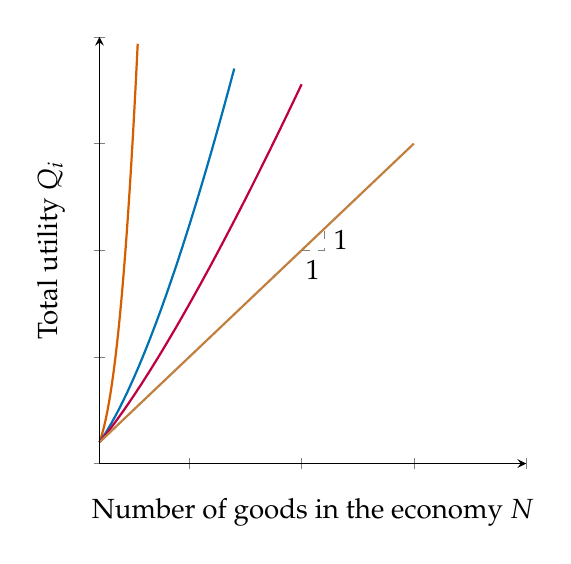
\begin{tikzpicture}
        \pgfmathsetmacro{\sigmaa}{1.5}
        \pgfmathsetmacro{\sigmab}{3}
        \pgfmathsetmacro{\sigmac}{5}
        
        \centering
        \begin{axis}[
            ylabel={Total utility $Q_i$},
            xlabel={Number of goods in the economy $N$},
            ymin=0, ymax=20,
            xmin=1, xmax=20,
            xticklabel=\empty,
            yticklabel=\empty,
            axis lines=left,
            enlargelimits=false,
            clip=false,
            axis on top,
            scaled x ticks=false,
            width=7cm, height=7cm,
            title style={font=\bfseries}
        ]
        
        % PPF: Q_C = (L/a_C) - (a_R/a_C) * Q_R
    
        
          \addplot[thick,red,  domain=1:2.7]
            {x^(\sigmaa / (\sigmaa -1))};
          \addplot[thick,blue, domain=1:7]
            {x^(\sigmab / (\sigmab -1)};
          \addplot[thick,purple, domain=1:10]
            {x^(\sigmac / (\sigmac -1)};
          \addplot[thick,brown,domain=1:15]
            {x};  

            \addplot[gray, dashed] coordinates
            {(10,10) (11,10) (11,11)};
            \node[anchor = north] at (axis cs: 10.5,10) {$1$};
            \node[anchor = west] at (axis cs: 11,10.5) {$1$};
            

        \end{axis}
    
    \end{tikzpicture}
            \caption{Love of variety with different elasticities: \textcolor{red}{$\sigma=1.5$, \textcolor{blue}{$\sigma=3$}, \textcolor{brown}{$\sigma=\infty$}}}
        \label{fig: ces-love}
    \end{figure}
\end{frame}


\begin{frame}{Love-of-variety: photographical representation}
\begin{figure}
    \centering
    \includegraphics[width=0.75\linewidth]{figs/yeltsin-variety.jpg}
    \caption{Boris Yeltsin, then president of the Russian Soviet Socialist Republic, visits America, 1989}
\end{figure}
\end{frame}


\begin{frame}{Rationing and lack of variety}
\begin{figure}
    \centering
    \includegraphics[width=0.6\linewidth]{figs/Libreta-Store.jpg}
    \caption{Rationing store in Cuba, 2012}
\end{figure}
\end{frame}

\section{Equilibrium}

\begin{frame}{Number of products $N^*$ in equilibrium}

\begin{wideitemize}
    \item How can we solve for the equilibrium number of firms $N^*$?

    \item<2-> By now, you probably now: we use some condition that makes supply = demand \\
    \qquad \textcolor{gray}{(``market clearing condition'')}

    \item<3-> In this case, we will use the labor market equilibrium

    \item<4-> Labor demand per firm: $\ell = \bar{f} +a^* q^*$; labor supply: $L_i$. In equilibrium:
    \onslide<5->{
    \begin{equation*}
        N^* (\bar{f} +a^* q^*) = N^* \left(\bar{f} +a^* (\sigma-1) \frac{\bar{f}}{a^*} \right) = L_i \iff N^* = \frac{L_i}{\sigma \bar{f}}
    \end{equation*} }
      \onslide<6->{ \blue{Intution}:

    \begin{itemize}
        \item large $L_i \rightarrow$ large market $\rightarrow$ the more goods/firms in equilibrium;
        \item large  $\bar{f} \rightarrow$ larger IRS $\rightarrow$ firms larger $\rightarrow$fewer firms in equilibrium.
        \item large $\sigma \rightarrow$ more substitutable goods $\rightarrow$ markups smaller $\rightarrow$ surviving firms have to sell more units to be able to pay for fixed costs $\rightarrow$ fewer firms in equilibrium.
    \end{itemize}
    }
    

\end{wideitemize}
    
\end{frame}

\begin{frame}{Labor market clearing}

    \begin{figure}[htp]
        \centering
        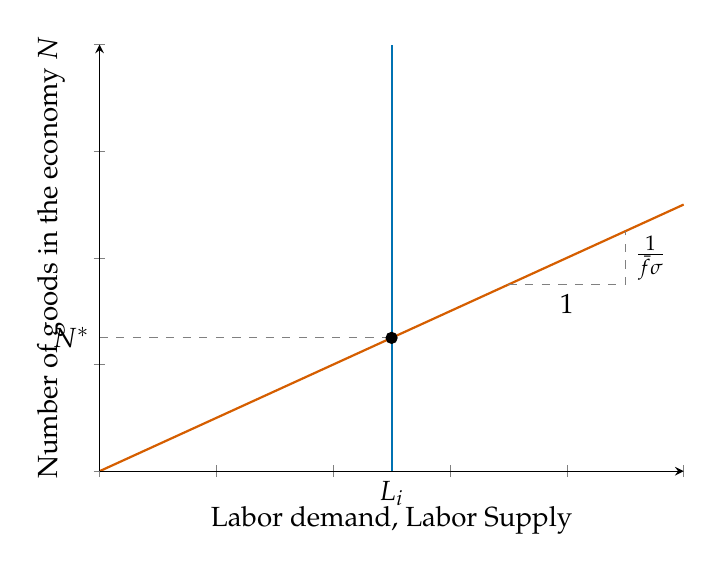
\begin{tikzpicture}
        \pgfmathsetmacro{\sigmaa}{2}
        \pgfmathsetmacro{\L}{2.5}
        \pgfmathsetmacro{\f}{1}
        \pgfmathsetmacro{\N}{\L / (\sigmaa * \f)}
        
        \centering
        \begin{axis}[
            xlabel={Labor demand, Labor Supply},
            ylabel={Number of goods in the economy $N$},
            ymin=0, ymax=4,
            xmin=0, xmax=5,
            yticklabel=\empty,
            xticklabel=\empty,
            axis lines=left,
            enlargelimits=false,
            clip=false,
            axis on top,
            scaled x ticks=false,
            width=9cm, height=7cm,
            title style={font=\bfseries}
        ]
        
        % PPF: Q_C = (L/a_C) - (a_R/a_C) * Q_R
    
        
          \addplot[thick,blue] coordinates
            {(\L,0) (\L,4)};
          \addplot[thick,red, domain=0:5]
            {1/(\f * \sigmaa) * x};
          \addplot[gray, dashed] coordinates
            {(0,\N) (\L,\N)};
            
            \addplot[only marks, mark=*, color=black, mark size=2pt] coordinates {(\L, \N)};      \node[anchor = east] at (axis cs:0,\N) {$N^*$};
            \node[anchor = north] at (axis cs:\L,0) {$L_i$};

            \pgfmathsetmacro{\xs}{\L + 1}
            \pgfmathsetmacro{\Ns}{1/(\f * \sigmaa) * \xs}
            \pgfmathsetmacro{\xsx}{\xs + 1}
            \pgfmathsetmacro{\Nsx}{1/(\f * \sigmaa) * \xsx}

            \addplot[gray, dashed] coordinates
            {(\xs,\Ns) (\xsx,\Ns) (\xsx,\Nsx)};
            \node[anchor = north] at (axis cs:{\xs + (\xsx - \xs)/2},\Ns) {$1$};
            \node[anchor = west] at (axis cs:\xsx,{\Ns + (\Nsx - \Ns)/2}) {$\frac{1}{\bar{f} \sigma}$};
        \end{axis}
    
    \end{tikzpicture}
            \caption{Labor market and number of firms equilibrium}
        \label{fig: labor-market}
    \end{figure}
\end{frame}

\begin{frame}{General Equilibrium}
\begin{wideitemize}
    \item What does it mean to find ``an equilibrium''?

    \item<2-> We solved for:
    \begin{itemize}
        \item prices: $\{p_i(\varphi),w_i\}$ \textcolor{gray}{{\scriptsize (wages $w_i=1$ are the num\'eraire of this economy)}}
        \item consumer demand choices: $\{p_i(\varphi)\}$
        \item firms production choices: $\{\ell\}$
        \item equilibrium number of firms: $\{N\}$
    \end{itemize}

    \item<3-> Such that:
    \begin{itemize}
        \item consumers maximize utility (behave optimally)
        \item firms maximize profits (behave optimally)
        \item factor markets clear: $L_i = N \times \ell^*$ 
        \item goods markets clear: $I_i = P_iQ_i = N\times p^* q^*$ \textcolor{gray}{{\scriptsize (check handout)}}
    \end{itemize}    
    
\end{wideitemize}
\end{frame}

\section{Opening up to trade}

\begin{frame}{Opening up to trade}
\begin{wideitemize}
    \item Two symmetric countries ($H$ and $F$)
    \item No trade barriers and shipping costs.
    \item<2-> Consumers now have preferences over domestic and foreign goods:
    \begin{itemize}
        \item $\Phi_H := \{ H_1, H_2, \cdots,H_{N_H} \}$: set of domestic goods.
        \item $\Phi_F := \{ F_1, F_2, \cdots,F_{N_F} \}$: set of foreign goods.
        \item $\Phi_i := \Phi_H \cup \Phi_F = \{ H_1, H_2, \cdots,H_{N_H}, F_1, F_2, \cdots,F_{N_F} \}$: all goods available in country $i$.
    \end{itemize}

    \item<3-> Preferences:
    \begin{eqnarray*}
        \max_{\{q_i(
    \varphi)\}_{\
    \varphi \in \Phi_i}} Q_i &\equiv& \left[ \underbrace{\sum_{\varphi \in \Phi_H } q_i(
    \varphi)^{\tfrac{\sigma-1}{\sigma}}}_{\text{home goods}} + \underbrace{\sum_{\varphi \in \Phi_F } q_i(
    \varphi)^{\tfrac{\sigma-1}{\sigma}}}_{\text{foreign goods }} \right]^{\tfrac{\sigma}{\sigma-1} } \\
    s.t. \qquad  P_i Q_i &=&\sum_{\varphi \in \Phi_i } p_i(\varphi) q_i(\varphi) \le I_i = w_i L_i 
\end{eqnarray*}
 

\end{wideitemize}
\end{frame}


\begin{frame}{Opening up to trade}
\begin{wideitemize}
    \item Everything else stays the same. Labor forces, and fixed costs are identical.
    
    \item Preferences are identical in each country, each firms face the same demand curve.
    
    \item<2-> The optimal price they will choose will be the same:

    \begin{equation*}
        p^* = \text{markup} \times \text{MC} = \frac{\sigma}{\sigma-1} \times MC
    \end{equation*}

    \item<3-> Fixed and marginal costs as the same as before $\rightarrow$ free entry condition $\pi_i(\varphi) =0$ pins down the same optimal quantity per firm:
    \begin{equation*}
        q^* = (\sigma-1) \times \frac{\bar{f}}{a^*}
    \end{equation*}

    \item<4-> How many firms exist in each country? Use the labor market clearing condition to find that:
    \begin{equation*}
        N^* = \frac{L_i}{\sigma \bar{f}}
    \end{equation*}
    

\end{wideitemize}
\end{frame}


\begin{frame}{Opening up to trade}
\begin{wideitemize}
    \item But wait... the same number of firms $N^*$ is active in each country as in autarky.
    
    \item<2-> So nothing changes? Not quite.

    \item<3-> With symmetric countries, integration the \emph{size of the market} in terms of available goods.
    
    \item<4-> That becomes clear once we evaluate what happens with welfare/utility:

\begin{eqnarray*}
         Q_i &\equiv& \left[ \sum_{\varphi \in \Phi_H } q_i(
    \varphi)^{\tfrac{\sigma-1}{\sigma}} +\sum_{\varphi \in \Phi_F } q_i(
    \varphi)^{\tfrac{\sigma-1}{\sigma}} \right]^{\tfrac{\sigma}{\sigma-1} } \\
    &=& \left[ N^* (q^*)^{\tfrac{\sigma-1}{\sigma}} +N^* (q^*)^{\tfrac{\sigma-1}{\sigma}} \right]^{\tfrac{\sigma}{\sigma-1} }\\
    &=& (2 N^*)^{\frac{\sigma}{\sigma-1}} q^*
\end{eqnarray*}

\end{wideitemize}
\end{frame}

\begin{frame}{Welfare after trade}
\begin{wideitemize}
    \item Consumers are better off after trade openness:

\begin{eqnarray*}
         Q_i^{\text{Trade}} = (2 N^*)^{\frac{\sigma}{\sigma-1}} q^* > (N^*)^{\frac{\sigma}{\sigma-1}} q^* =Q_i^{\text{Autarky}}
\end{eqnarray*}

\item With identical countries, half of the new entrants locate in $H$ and half in $F$

\item Wach country \emph{hosts} the same number of firms as before ($N^{*}=L/(\sigma\bar f)$)...

\item ...but consumers in both countries can now purchase \emph{all} $2N^*$ varieties.

\end{wideitemize}
\end{frame}

\begin{frame}{Trade equilibrium}

\begin{wideitemize}
    \item Every firm sells one identical good to \emph{both} markets.
    
    \item<2-> Country $H$ exports the set of varieties it produces and imports the set produced in $F$, and vice-versa.
    
    \item<3-> Because the two sets have equal value, bilateral trade is balanced:

    \begin{equation*}
        \text{Exports}_{H\to F} = \text{Imports}_{F\to H}
    \end{equation*}

    \item<4-> But why does trade even happen in this world?
    
\end{wideitemize}
    
\end{frame}

\begin{frame}{Interindustry trade}

\begin{wideitemize}
    \item In the other models we saw (Ricardian, SFM or HO) identical identical countries would have \blue{no} reason to trade

    \item Gains from trade hing on cross-country differences and differences in relative prices

    \item The Krugman model showcases \blue{horizontal intra-industry trade} that arises \blue{even though the countries are identical}
    
    \item Gains from trade come from the \blue{love-of-variety} and the ability of increasing-returns firms to cover fixed costs in a larger market.
    
\end{wideitemize}
    
\end{frame}

\begin{frame}{Takeaway}

Trade in the Krugman model is fundamentally different from comparative advantage trade: \blue{it is horizontal and survives even when countries look exactly alike}.  Integration doubles the menu of goods, lowers the price index, and raises welfare without changing firm size, wages, or the markup.

    
\end{frame}





%----------------------------------------------------------------------%
%----------------------------------------------------------------------%


\end{document}
